\documentclass[10pt]{beamer}
% \documentclass[handout,10pt]{beamer}
\usepackage{my_style}

\title[Math/CS 375]{Lecture 10 - A}
\subtitle{\S 6.1 Splines }


\begin{document}
% -------------------------------------------------
\begin{frame}
  \titlepage
\end{frame}
% -------------------------------------------------
\begin{frame}{Goals}
We will answer these questions:\\[3mm]
\begin{itemize}
    \item What are splines? In what way are they advantageous over standard polynomial interpolation?

    \item What makes a spline different from a piecewise polynomial? 

    \item Is a degree 1 spline unique? 

    \item What are the conditions on a degree 2 spline? Is it unique?
\end{itemize}
\end{frame}

%%%%%%%%%%%%%%%%%%%%%%%%%%%%%%%%%%%%%%%%%%%%%%%%%%%%%%%%%%%%%%%%%%%%%%%%
\sectionframe{Problems with Polynomial Interpolation}
%%%%%%%%%%%%%%%%%%%%%%%%%%%%%%%%%%%%%%%%%%%%%%%%%%%%%%%%%%%%%%%%%%%%%%%%

\begin{frame}{Runge's Phenomenon}


\begin{block}{Runge's Phenomenon}
\begin{itemize}
\item Suppose we interpolate large data set using \textbf{a single high-degree polynomial}
\item  Polynomial interpolation at equally spaced points can exhibit large oscillations at the boundaries

\end{itemize}
\end{block}

\vspace{2mm}

\begin{block}{Example - Try interpolation on this data set}
\begin{figure}
    \centering
    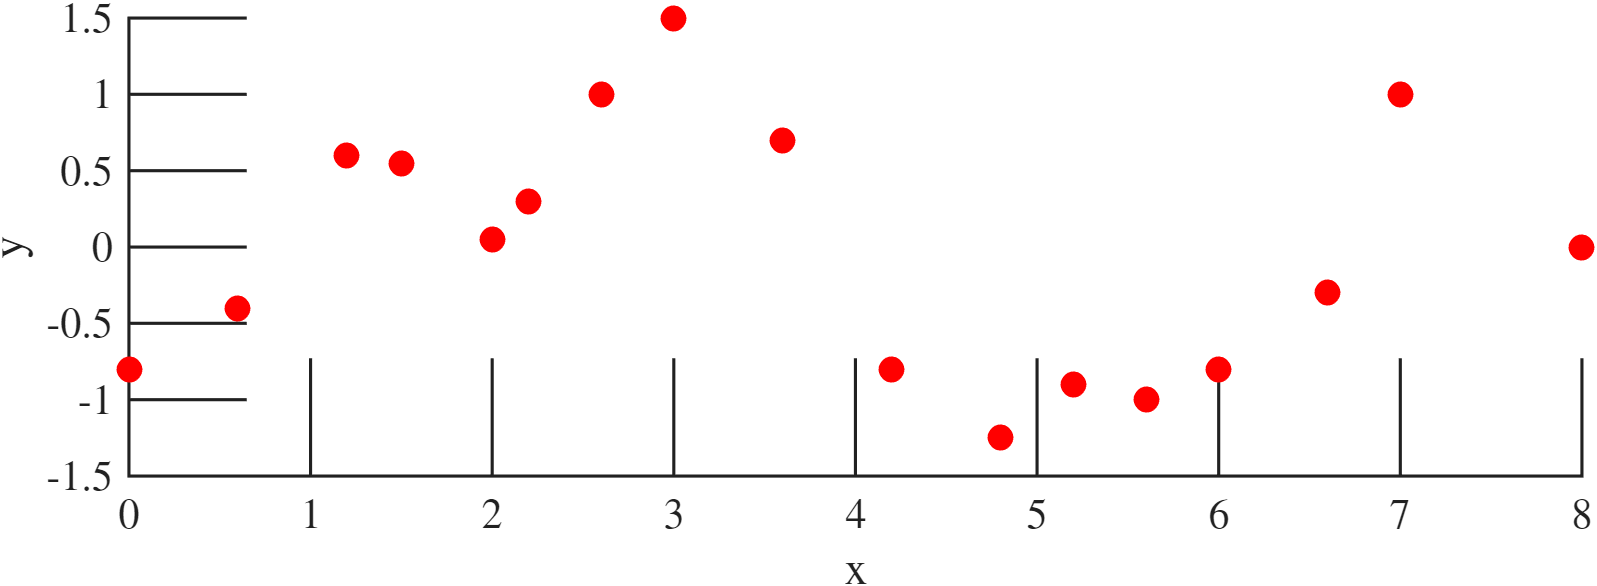
\includegraphics[width=0.6\linewidth]{figs/problem1.png}
\end{figure}
\end{block}

\end{frame}

%%%%%%%%%%%%%

\begin{frame}{Runge's Phenomenon}
\begin{figure}
    \centering
    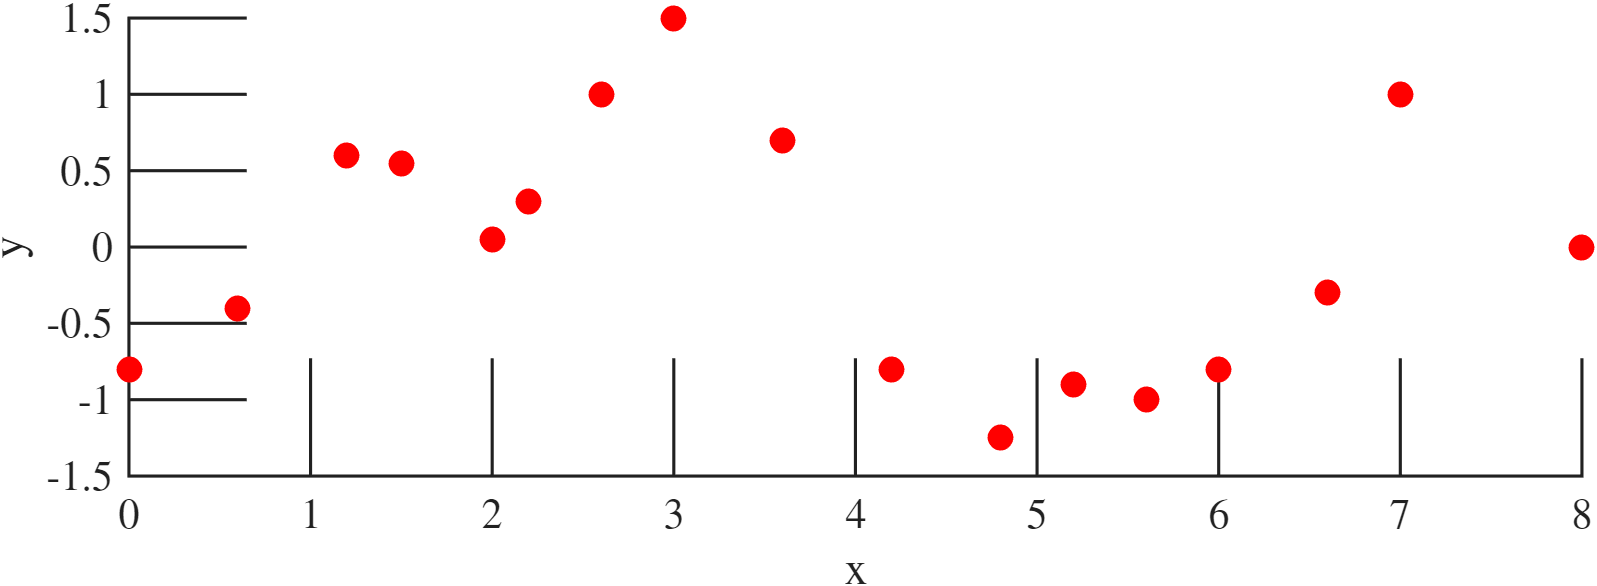
\includegraphics[width=0.65\linewidth]{figs/problem1.png}
\end{figure}
\begin{figure}
    \centering
    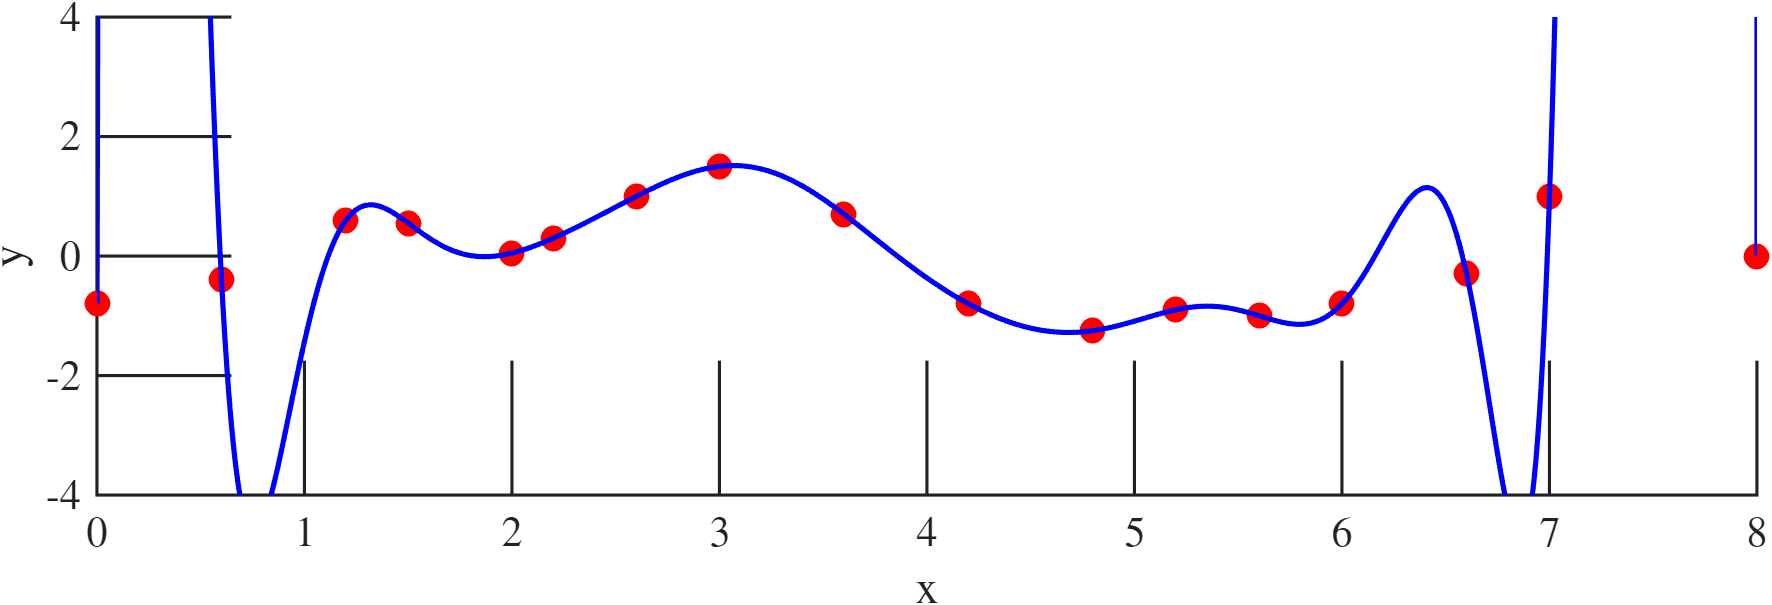
\includegraphics[width=0.65\linewidth]{figs/problem1b.png}
\end{figure}

\keyidea{
Fitting a high-degree polynomial on a data set can lead to disappointing results.
}
\end{frame}

%%%%%%%%%%%%%

\begin{frame}{Non-differentiable Functions}
    \begin{itemize}
    \item Real data is often:, noisy, piecewise-defined, or non-smooth
    \item But a  polynomial is infinitely differentiable
    \item This forces \textbf{artificial smoothness} everywhere
\end{itemize}

\begin{figure}
    \centering
    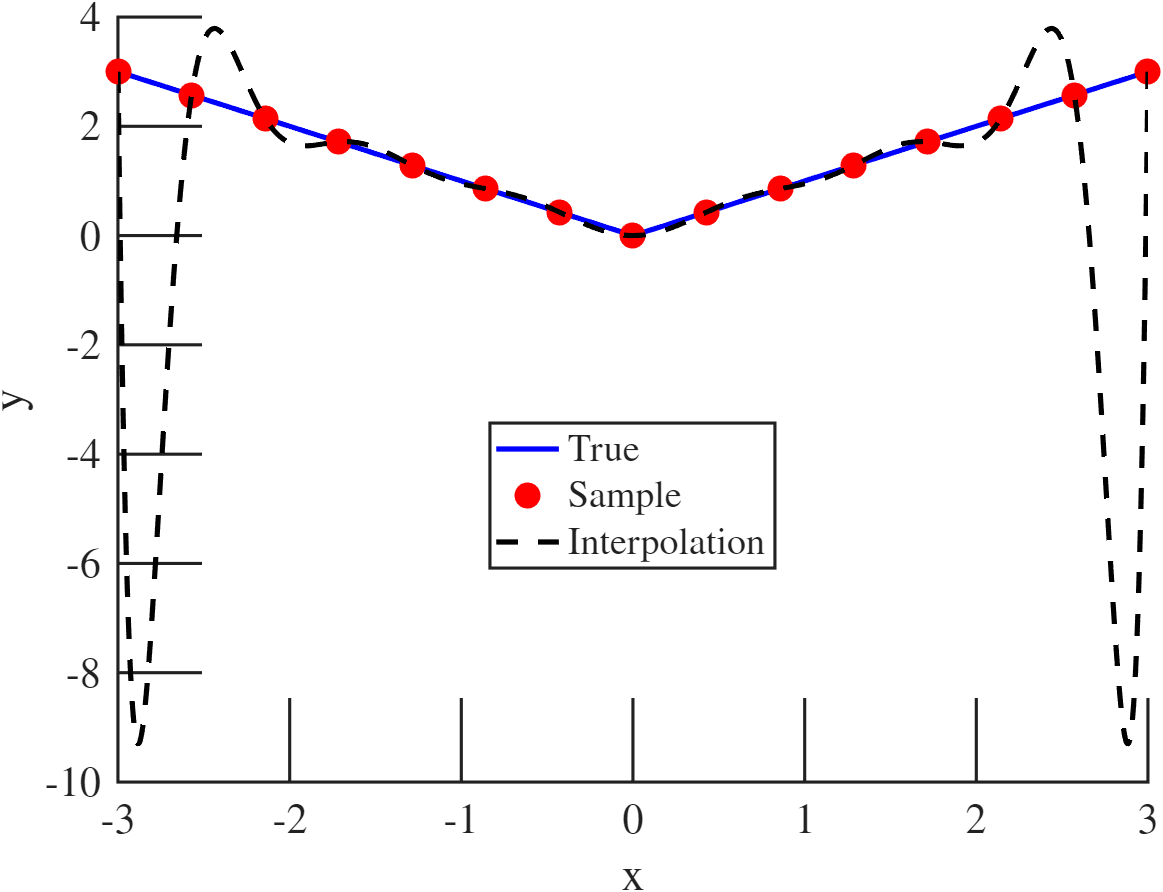
\includegraphics[width=0.5\linewidth]{figs/problem2.png}
    \caption{Interpolation on $f(x) = |x|$ has large errors at the boundaries}
\end{figure}

\end{frame}

%%%%%%%%%%%%%

\begin{frame}{Instability}
    \begin{itemize}
    \item Polynomial interpolation is a \textbf{global} method.
    \item Changing one data point affects the entire polynomial.
\end{itemize}


\begin{figure}
    \centering
    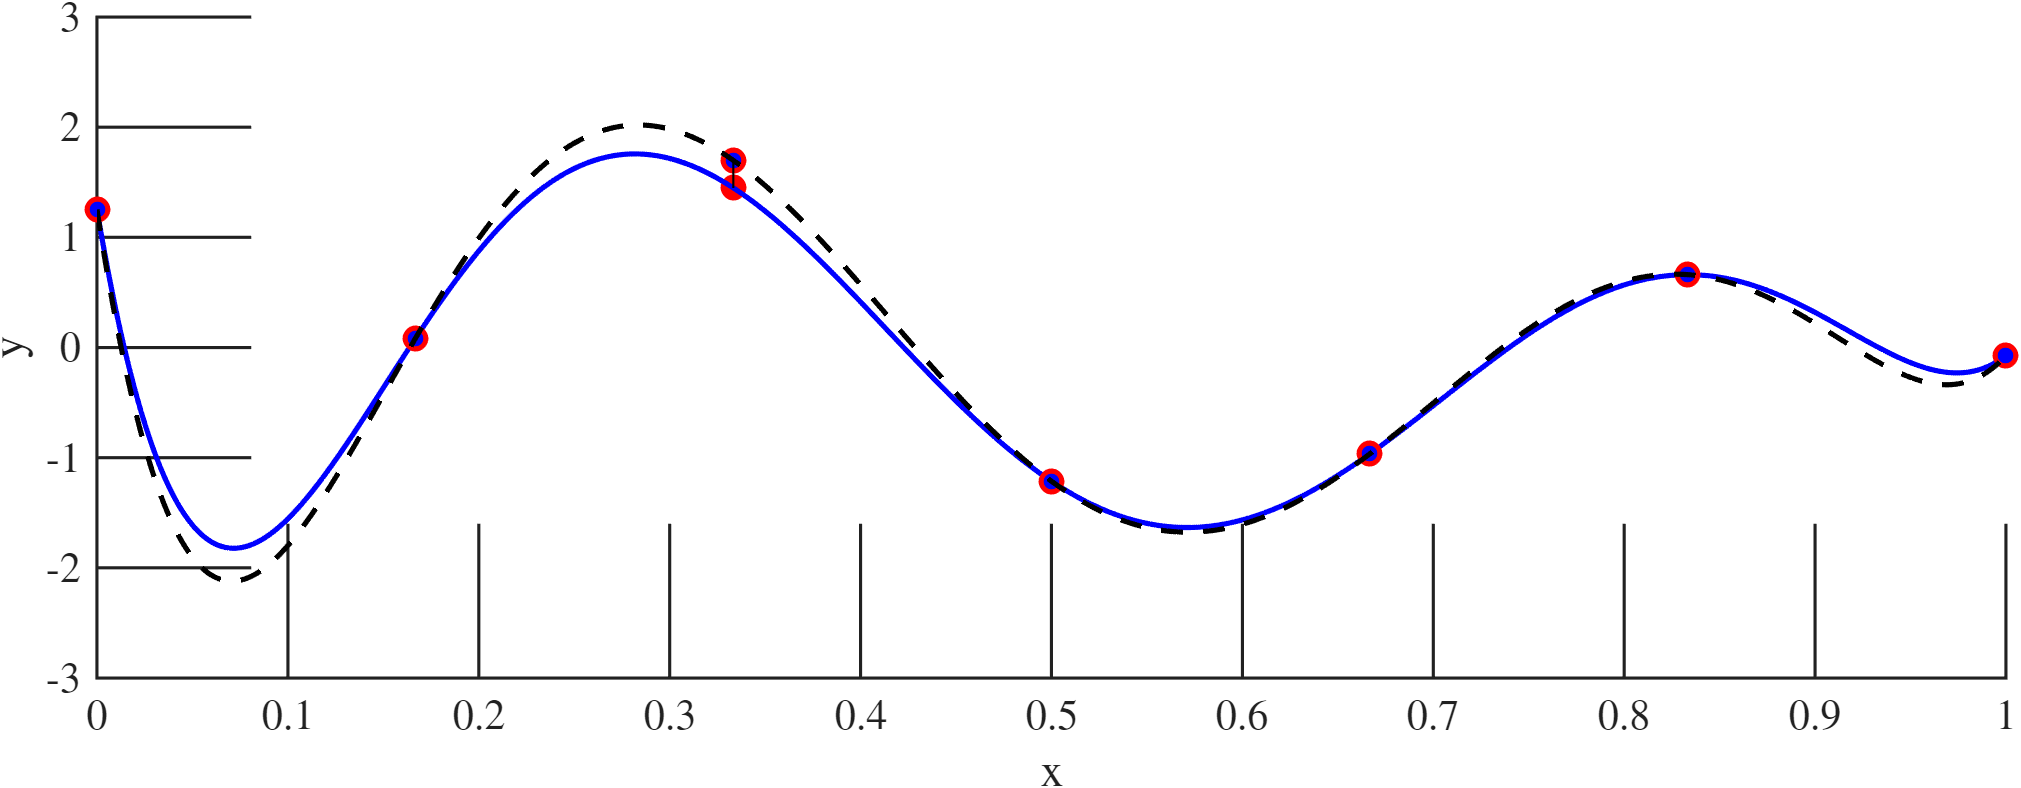
\includegraphics[width=0.7\linewidth]{figs/problem3.png}
    \caption{A local change in data causes global error}
\end{figure}

\begin{block}{Instability}
A small local perturbation affects the entire interpolation.
\end{block}

\end{frame}

%%%%%%%%%%%%%

\begin{frame}{The Solution}

\begin{block}{What we tried}
    Create \emph{one big polynomial} $p(x)$ to fit the data $(x_i,y_i)$.
\end{block}

\begin{block}{Issues}
    \begin{itemize}
        \item Polynomial degree grows with number of data points
        \item Runge's phenomenon 
        \item Not good for non-differentiable functions 
        \item Local change in data causes global changes
    \end{itemize}
\end{block}
\vspace{3mm}

\onslide<2>{
\begin{block}{The Fix}
\textbf{splines} - create \emph{multiple little polynomials} 
\end{block}
}



\end{frame}

%%%%%%%%%%%%%%%%%%%%%%%%%%%%%%%%%%%%%%%%%%%%%%%%%%%%%%%%%%%%%%%%%%%%%%%%
\sectionframe{Splines}
%%%%%%%%%%%%%%%%%%%%%%%%%%%%%%%%%%%%%%%%%%%%%%%%%%%%%%%%%%%%%%%%%%%%%%%%
\begin{frame}
\frametitle{Why Splines?}
\begin{columns}
\begin{column}{0.45\textwidth}
\begin{center}
  \pgfimage[width=2.5cm]{./figs/truetype_3}
\end{center}
\begin{center}
  \pgfimage[width=2.5cm]{./figs/utah_teapot}
\end{center}
\begin{center}
  \pgfimage[width=2.5cm]{./figs/spline1}
\end{center}
\end{column}
\begin{column}{0.45\textwidth}
\begin{itemize}
  \item Used for smooth lines and surfaces\\[3mm]
  \vfill 
  \item Truetype fonts, smooth textures\\[3mm]
  \vfill 
  \item Use low-degree \textbf{piecewise polynomials}\\[3mm]
  \vfill 
\end{itemize}
\end{column}
\end{columns}
\end{frame}
%%%%%%%%%%%%%%%%%%%%%%%%%%%%%%%%%%%%%%%%%%%%%%%%%%%%%%%%%%%%%%%%%%%%%%%%

\begin{frame}{Piecewise Polynomial}
A function $f(x)$ is a \textbf{piecewise polynomial} on $[a,b]$ if
there exists a (finite) partition $P$ of $[a,b]$ such that $f(x)$ is a
polynomial on each $[t_i,t_{i+1}]\in P$.

\begin{block}{Example}
\begin{equation*}
  f(x) = \begin{cases}
x^3 & x \in [0,1]\\
x & x \in (1,2)\\
3 & x \in [2,3]\\
\end{cases}
\end{equation*}
\end{block}
\begin{center}
  \pgfimage[width=4.5cm]{./figs/pwpoly}
\end{center}
\end{frame}
%%%%%%%%%%%%%%%%%%%%%%%%%%%%%%%%%%%%%%%%%%%%%%%%%%%%%%%%%%%%%%%%%%%%%%%%

\begin{frame}{Piecewise Polynomial vs. Spline}

\question{What makes a spline different from a piecewise function?}

{
\define{Spline}{
A \textbf{spline function} $S(x)$ is a piecewise function consisting of polynomials joined together with certain "smoothness" conditions. 
$$
S(x) = \begin{dcases}
    S_0(x), &x\in[t_0,t_1]\\
    S_1(x), &x\in[t_1,t_2]\\
      \quad\vdots  &\quad \vdots\\
      S_{n-1}(x), & x\in[t_{n-1},t_n]
\end{dcases}
$$
}
}
\begin{itemize}
    \item Splines consist of polynomials of the same degree
    \item Must interpolate a data set $(x_i,y_i)$
    \item Must satisfy a global "smoothness" condition
\end{itemize}

% \method{Spline Interpolation}{Set of points $(t_i,y_i)$, Degree of smoothness.}{Continuous piecewise polynomial $S(x)$}{Degree of the polynomial is fixed, yet we can still satisfy $S(t_i)=y_i$ for all points}
\end{frame}

%%%%%%%%%%%%%%%%%%%%%%%%%%%%%%%%%%%%%%%%%%%%%%%%%%%%%%%%%%%%%%%%%%%%%
\begin{frame}[shrink]{Notations}
\begin{block}{Data Set}
    Use $t$ and $y$ for the given data set
    $$
        (t_i,y_i),\quad \text{for }i=0,1,2,\dots, n
    $$
\end{block}

\begin{block}{Objective}
    Construct spline function $S(x)$ such that 
    $$
        S(t_i)=y_i
    $$
    and is composed of polynomials
    $$
        S_i(x),\quad \text{for } x\in[t_i,t_{i+1})
    $$
\end{block}

\method{Spline Interpolation}{Set of points $(t_i,y_i)$, Degree of smoothness.}{Continuous piecewise polynomial $S(x)$}{Degree of the polynomial is fixed, yet we can still satisfy $S(t_i)=y_i$ for all points}

\end{frame}

%%%%%%%%%%%%%%%%%%%%%%%%%%%%%%%%%%%%%%%%%%%%%%%%%%%%%%%%%%%%%%%%%%%%%
\sectionframe{Degree One Spline}
%%%%%%%%%%%%%%%%%%%%%%%%%%%%%%%%%%%%%%%%%%%%%%%%%%%%%%%%%%%%%%%%%%%%%

%%%%%%%%%%%%%%%%%%%%%%%%%%%%%%%%%%%%%%%%%%%
\begin{frame}{The Simplest Piecewise Interpolant}

\question{
What is the simplest piecewise function that interpolates these data?
}

\begin{center}
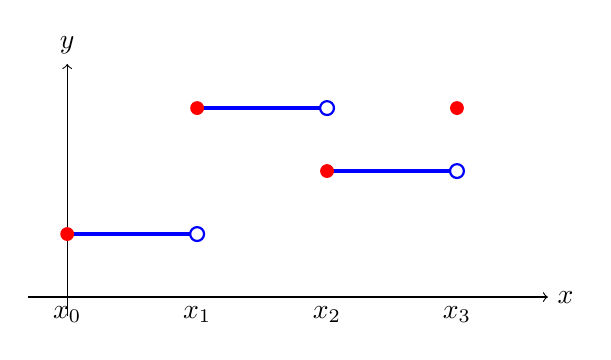
\begin{tikzpicture}[x=1.65cm,y=0.8cm]
    % Axes
    \draw[->] (-0.3,0) -- (3.7,0) node[right] {$x$};
    \draw[->] (0,-0.3) -- (0,3.7) node[above] {$y$};

    % Degree-zero interpolant
    \only<2->{
        \draw[blue,very thick] (0,1) -- (1,1);
        \draw[blue,very thick] (1,3) -- (2,3);
        \draw[blue,very thick] (2,2) -- (3,2);

        % Excluded right endpoints
        \foreach \x/\y in {1/1,2/3,3/2}{
            \draw[blue,thick,fill=white]
                (\x,\y) circle (2.5pt);
        }
    }

    % Data points
    \foreach \x/\y/\i in {0/1/0,1/3/1,2/2/2,3/3/3}{
        \fill[red] (\x,\y) circle (2.5pt);
        \node[below] at (\x,0) {$x_{\i}$};
    }
\end{tikzpicture}
\end{center}

% \onslide<2->{
% \begin{block}{Degree 0: Piecewise Constant}
% \[
% S_0(x)=
% \begin{cases}
%     y_0, & x_0\le x<x_1,\\
%     y_1, & x_1\le x<x_2,\\
%     y_2, & x_2\le x<x_3,\\
%     y_3, & x=x_3.
% \end{cases}
% \]
% \end{block}
% }
\begin{itemize}
    \item This is called a \textbf{Degree Zero Spline}
\end{itemize}


\end{frame}

%%%%%%%%%%%%%%%%%%%%%%%%%%%%%%%%%%%%%%%%%%%
\begin{frame}{What's the next simplest idea?}

\begin{itemize}
    \item Degree Zero splines has \textbf{jumps}.
\end{itemize}

\begin{center}
\begin{tikzpicture}[x=1.65cm,y=0.8cm]
    % Axes
    \draw[->] (-0.3,0) -- (3.7,0) node[right] {$x$};
    \draw[->] (0,-0.3) -- (0,3.7) node[above] {$y$};

    % Old constant pieces
    \only<1>{
        \draw[blue,very thick] (0,1) -- (1,1);
        \draw[blue,very thick] (1,3) -- (2,3);
        \draw[blue,very thick] (2,2) -- (3,2);

        \foreach \x/\y in {1/1,2/3,3/2}{
            \draw[blue,thick,fill=white]
                (\x,\y) circle (2.5pt);
        }
    }

    % Replace with linear pieces
    \only<2->{
        \draw[blue,very thick] (0,1) -- (1,3) -- (2,2) -- (3,3);
    }

    % Data points
    \foreach \x/\y/\i in {0/1/0,1/3/1,2/2/2,3/3/3}{
        \fill[red] (\x,\y) circle (2.5pt);
        \node[below] at (\x,0) {$x_{\i}$};
    }
\end{tikzpicture}
\end{center}

\onslide<2->{
\begin{block}{Degree One: Piecewise Linear}
Connect consecutive data points with straight lines.
\begin{itemize}
    \item Interpolates the data
    \item All pieces are polynomials
    \item Globally continuous
\end{itemize}
\end{block}
}


\end{frame}

% \begin{frame}{Continuity}
% \begin{itemize}
%   \item The lowest degree of "smoothness" is just $C^0$ continuity

% \begin{center}
%   \pgfimage[width=5.8cm]{./figs/pwpoly}
%   \pgfimage[width=5.0cm]{./figs/spline2}
% \end{center}
%     \item Function on the right is called a \textbf{first-degree spline}
% \end{itemize}
% \end{frame}
%%%%%%%%%%%%%%%%%%%%%%%%%%%%%%%%%%%%%%%%%%%%%%%%%%%%%%%%%%%%%%%%%%%%%%%%

\begin{frame}{First-Degree Spline}

\define{First-Degree Spline }{
A function $S(x)$ is a \textbf{spline of degree 1} if it satisfies all of the following:
\begin{enumerate}
  \item The domain of $S(x)$ is an interval $[a,b]$
  \item $S(x)$ is continuous on $[a,b]$
  \item There is a partition $a=t_0<t_1<\dots<t_n=b$ such that $S(x)$ is
\emph{linear} on each subinterval $[t_i,t_{i+1}]$.
\end{enumerate}
}
\begin{itemize}
    \item First-degree spline is made up of lines that are connected end-to-end
\end{itemize}
\begin{example}
Is this function a spline of degree 1?
\begin{equation*}
  f(x) = \begin{cases}
  x & x \in [-1,0]\\
  0 & x \in (0,1)\\
  2x-2 & x \in [1,2]\\
\end{cases}
\end{equation*}
\end{example}
\end{frame}
%%%%%%%%%%%%%%%%%%%%%%%%%%%%%%%%%%%%%%%%%%%%%%%%%%%%%%%%%%%%%%%%%%%%%%%%

\begin{frame}{Degree 1 Spline}
\begin{columns}
\begin{column}{0.45\textwidth}
\begin{example}
\begin{equation*}
  f(x) = \begin{cases}
  x & x \in [-1,0]\\
  0 & x \in (0,1)\\
  2x-2 & x \in [1,2]\\
\end{cases}
\end{equation*}
\end{example}
\end{column}
\begin{column}{0.45\textwidth}
\begin{center}
  \pgfimage[width=5.5cm]{./figs/spline3}
\end{center}
\end{column}
\end{columns}
\begin{itemize}
    \item Is it continuous at $x=0$? yes 
    \item Is it continuous at $x=1$? yes 
    \item Is each component a line? yes 
    \item Therefore $f(x)$ a first-degree spline
\end{itemize}
\end{frame}
%%%%%%%%%%%%%%%%%%%%%%%%%%%%%%%%%%%%%%%%%%%%%%%%%%%%%%%%%%%%%%%%%%%%%%%%

\begin{frame}{Formula for $S_i(x)$}

There are three conditions on $S_i$
\begin{enumerate}
  \item $S_i(t_i) = y_i$
  \item $S_i(t_{i+1})=y_{i+1}$
  \item $S_i(x) = m(x-x_0) +y_0$ 
\end{enumerate}

\cols{  
Write $S_i(x)$ in point-slope form
\begin{align*}
  S_i(x) & = y_0 + m(x-x_0)\\
         & = y_i + \frac{y_{i+1}-y_i}{t_{i+1}-t_i}(x-t_i)
\end{align*}
}{
\begin{center}
   
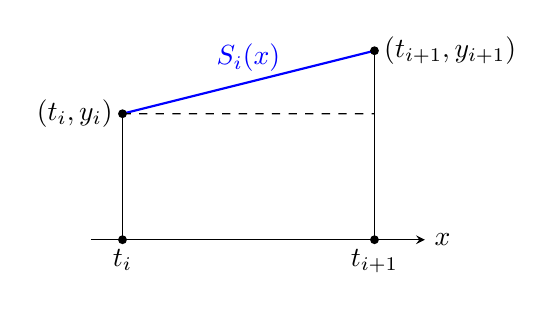
\begin{tikzpicture}[scale=0.8,>=stealth]
% coordinates
\coordinate (ti)  at (0,0);
\coordinate (tip) at (4,0);

\coordinate (yi)  at (0,2);
\coordinate (yip) at (4,3);

% axes
\draw[->] (-0.5,0) -- (4.8,0) node[right] {$x$};

% vertical lines
\draw (ti) -- (yi);
\draw (tip) -- (yip);

% spline segment
\draw[thick,blue] (yi) -- (yip) node[midway,above] {$S_i(x)$};

% dashed horizontal guide
\draw[dashed] (yi) -- (4,2);

% points
\fill (ti) circle (2pt);
\fill (tip) circle (2pt);
\fill (yi) circle (2pt);
\fill (yip) circle (2pt);

% labels
\node[below] at (ti) {$t_i$};
\node[below] at (tip) {$t_{i+1}$};

\node[left]  at (yi) {$(t_i,y_i)$};
\node[right] at (yip) {$(t_{i+1},y_{i+1})$};
\end{tikzpicture}
\end{center}
s}

\end{frame}

%%%%%%%%%%%%%%%%%%%%%%%%%%%%

\begin{frame}{Example: Degree-1 Spline}

\begin{example}
Construct the \textbf{degree-1 spline} that interpolates the data
\[
(0,1), \quad
(1,3), \quad
(3,2).
\]
\end{example}

\begin{itemize}
    \item On the interval $[0,1]$ 
\[
m_0 = \frac{3-1}{1-0} = 2
\]
Thus,
\[
S_0(x) = 1 + 2x, \quad 0 \le x \le 1.
\]


\item On the interval $[1,3]$
Slope:
\[
m_1 = \frac{2-3}{3-1} = -\frac12
\]
Thus,
\[
S_1(x) = 3 - \tfrac12(x-1), \quad 1 \le x \le 3.
\]

% \begin{block}{Final spline}
% \[
% S(x) =
% \begin{cases}
% 1 + 2x, & 0 \le x \le 1,\\[2mm]
% 3 - \tfrac12(x-1), & 1 \le x \le 3.
% \end{cases}
% \]
% \end{block}
\end{itemize}


\end{frame}



%%%%%%%%%%%%%%%%%%%%%%%%%%%%%%%%%%%%%%%%%%%%%%%%%%%%%%%%%%%%%%%%%%%%%%%%
\sectionframe{Constraints vs. Unknowns}
%%%%%%%%%%%%%%%%%%%%%%%%%%%%%%%%%%%%%%%%%%%%%%%%%%%%%%%%%%%%%%%%%%%%%%%%

\begin{frame}{Number of Unknowns}
\begin{center}
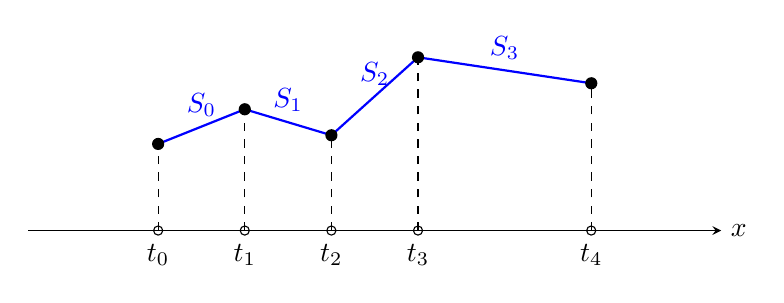
\begin{tikzpicture}[scale=1.1,>=stealth]
% Axis
\draw[->] (-1.5,0) -- (6.5,0) node[right] {$x$};

% Knot positions
\foreach \x/\label in {0/t_0,1/t_1,2/t_2,3/t_3,5/t_4} {
    \draw (\x,0) circle (1.5pt);
    \node[below] at (\x,-0.05) {$\label$};
}

% Points (ti, yi)
\coordinate (P0) at (0,1);
\coordinate (P1) at (1,1.4);
\coordinate (P2) at (2,1.1);
\coordinate (P3) at (3,2.0);
\coordinate (P4) at (5,1.7);

% Vertical dashed lines
\foreach \p in {P0,P1,P2,P3,P4} {
    \draw[dashed] (\p |- 0,0) -- (\p);
}

% Spline segments
\draw[thick,blue] (P0) -- (P1) node[midway,above] {$S_0$};
\draw[thick,blue] (P1) -- (P2) node[midway,above] {$S_1$};
\draw[thick,blue] (P2) -- (P3) node[midway,above] {$S_2$};
\draw[thick,blue] (P3) -- (P4) node[midway,above] {$S_3$};

% Data points
\foreach \p in {P0,P1,P2,P3,P4} {
    \fill (\p) circle (2pt);
}

\end{tikzpicture}
\end{center}
\begin{itemize}
    \item Suppose there are 5 nodes $(t_i,y_i)$ for $i=0,1,2,3,4$
    \item Then there are $n=4$ subintervals 
    \question{
    How many unknown coefficients are needed to specify the spline $S(x)$?
    }
\end{itemize}
\end{frame}

%%%%%%%%%%%%%%%%%%%%%%%%%%%%%%%%%%%%%%

\begin{frame}{Number of Unknowns}
\begin{center}
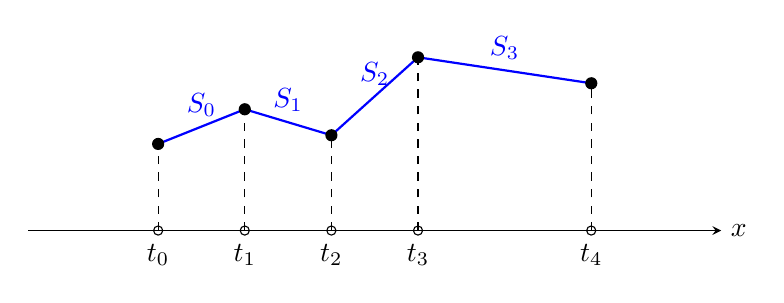
\begin{tikzpicture}[scale=1.1,>=stealth]
% Axis
\draw[->] (-1.5,0) -- (6.5,0) node[right] {$x$};

% Knot positions
\foreach \x/\label in {0/t_0,1/t_1,2/t_2,3/t_3,5/t_4} {
    \draw (\x,0) circle (1.5pt);
    \node[below] at (\x,-0.05) {$\label$};
}

% Points (ti, yi)
\coordinate (P0) at (0,1);
\coordinate (P1) at (1,1.4);
\coordinate (P2) at (2,1.1);
\coordinate (P3) at (3,2.0);
\coordinate (P4) at (5,1.7);

% Vertical dashed lines
\foreach \p in {P0,P1,P2,P3,P4} {
    \draw[dashed] (\p |- 0,0) -- (\p);
}

% Spline segments
\draw[thick,blue] (P0) -- (P1) node[midway,above] {$S_0$};
\draw[thick,blue] (P1) -- (P2) node[midway,above] {$S_1$};
\draw[thick,blue] (P2) -- (P3) node[midway,above] {$S_2$};
\draw[thick,blue] (P3) -- (P4) node[midway,above] {$S_3$};

% Data points
\foreach \p in {P0,P1,P2,P3,P4} {
    \fill (\p) circle (2pt);
}

\end{tikzpicture}
\end{center}
\begin{itemize}
    \item Each component has the form 
    $$S_i(x) = m_ix + b_i,\qquad i=1,2,3,4$$
    \item Therefore there are $4\times2 =$ \textbf{8 unknowns}
    \begin{block}{General Number of Unknowns}
        In general, a first-degree spline with $n+1$ nodes will require computing $2n$ unknown coefficients.
    \end{block}
\end{itemize}
\end{frame}



%%%%%%%%%%%%%%%%%%%%%%%%%%%%%%%%%%%%%%

\begin{frame}{Number of Constraints}
\begin{center}
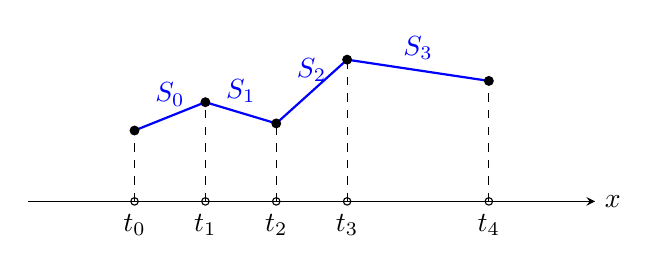
\begin{tikzpicture}[scale=0.9,>=stealth]
% Axis
\draw[->] (-1.5,0) -- (6.5,0) node[right] {$x$};

% Knot positions
\foreach \x/\label in {0/t_0,1/t_1,2/t_2,3/t_3,5/t_4} {
    \draw (\x,0) circle (1.5pt);
    \node[below] at (\x,-0.05) {$\label$};
}

% Points (ti, yi)
\coordinate (P0) at (0,1);
\coordinate (P1) at (1,1.4);
\coordinate (P2) at (2,1.1);
\coordinate (P3) at (3,2.0);
\coordinate (P4) at (5,1.7);

% Vertical dashed lines
\foreach \p in {P0,P1,P2,P3,P4} {
    \draw[dashed] (\p |- 0,0) -- (\p);
}

% Spline segments
\draw[thick,blue] (P0) -- (P1) node[midway,above] {$S_0$};
\draw[thick,blue] (P1) -- (P2) node[midway,above] {$S_1$};
\draw[thick,blue] (P2) -- (P3) node[midway,above] {$S_2$};
\draw[thick,blue] (P3) -- (P4) node[midway,above] {$S_3$};

% Data points
\foreach \p in {P0,P1,P2,P3,P4} {
    \fill (\p) circle (2pt);
}

\end{tikzpicture}
\end{center}
\question{How many constraints or equations are enforced on the spline $S(x)$ for the function above?}
\begin{itemize}
    \item Constraint on $S_0(x)$: $S_0(t_0)=y_0$ and $S_0(t_1)=y_1$
    \item Constraint on $S_1(x)$: $S_1(t_1)=y_1$ and $S_1(t_2)=y_2$
    \item Constraint on $S_2(x)$: $S_2(t_2)=y_2$ and $S_2(t_3)=y_3$
    \item Constraint on $S_3(x)$: $S_3(t_3)=y_3$ and $S_3(t_4)=y_4$ 
\end{itemize}
\end{frame}

%%%%%%%%%%%%%%%%%%%%%%%%%%%%%%%%%%%%%%
%%%%%%%%%%%%%%%%%%%%%%%%%%%%%%%%%%%%%%

\begin{frame}{Number of Constraints}
\begin{center}
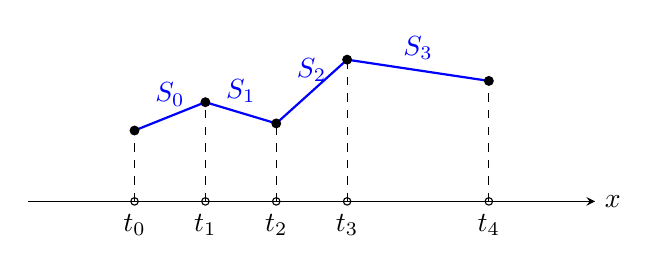
\begin{tikzpicture}[scale=0.9,>=stealth]
% Axis
\draw[->] (-1.5,0) -- (6.5,0) node[right] {$x$};

% Knot positions
\foreach \x/\label in {0/t_0,1/t_1,2/t_2,3/t_3,5/t_4} {
    \draw (\x,0) circle (1.5pt);
    \node[below] at (\x,-0.05) {$\label$};
}

% Points (ti, yi)
\coordinate (P0) at (0,1);
\coordinate (P1) at (1,1.4);
\coordinate (P2) at (2,1.1);
\coordinate (P3) at (3,2.0);
\coordinate (P4) at (5,1.7);

% Vertical dashed lines
\foreach \p in {P0,P1,P2,P3,P4} {
    \draw[dashed] (\p |- 0,0) -- (\p);
}

% Spline segments
\draw[thick,blue] (P0) -- (P1) node[midway,above] {$S_0$};
\draw[thick,blue] (P1) -- (P2) node[midway,above] {$S_1$};
\draw[thick,blue] (P2) -- (P3) node[midway,above] {$S_2$};
\draw[thick,blue] (P3) -- (P4) node[midway,above] {$S_3$};

% Data points
\foreach \p in {P0,P1,P2,P3,P4} {
    \fill (\p) circle (2pt);
}
\end{tikzpicture}
\end{center}

\begin{itemize}
    \item For each of the $n=4$ components $S_i(x)$, we have $two$ constraints 
    \item Therefore there are $4\times2 = $\textbf{8 constraints}
    
    \begin{block}{General Number of Unknowns}
        In general, a first-degree spline with $n+1$ nodes will have $2n$ number of constraints.
    \end{block}
    
\end{itemize}
\end{frame}


%%%%%%%%%%%%%%%%%%%%%%%%%%%%%%%%%%
\begin{frame}{Summary for Degree 1 Splines}

\begin{block}{Counting Unknowns}
\begin{itemize}
    \item There are $n$ subintervals and each piece is linear:
    \[
        S_i(x) = m_i x + b_i
    \]
    \item This gives \textbf{$2n$ unknown coefficients}
\end{itemize}
\end{block}

\begin{block}{Counting Constraints}
\begin{itemize}
    \item Each spline piece must interpolate its two endpoints
    \item This enforces \textbf{$2n$ equations}
\end{itemize}
\end{block}


\keyidea{
Since we have 
\begin{center}
\fbox{\parbox{0.75\textwidth}{
\centering
\textbf{Number of unknowns = number of constraints}
}}
\end{center}
the first-degree spline $S(s)$ is unique.
}

% \onslide<2>{
% \begin{alertblock}{What changes for higher-degree splines?}
% \begin{itemize}
%     \item More coefficients per interval
%     \item Interpolation alone is no longer sufficient
%     \item We will need \textbf{smoothness conditions}
% \end{itemize}
% \end{alertblock}
% }
\end{frame}
%%%%%%%%%%%%
%%%%%%%%%%%%%%%%%%%%%%%%%%%%%%
\begin{frame}{Continuity Condition}

\define{First-Degree Spline }{
A function $S(x)$ is a \textbf{spline of degree 1} if it satisfies all of the following:
\begin{enumerate}
  \item The domain of $S(x)$ is an interval $[a,b]$
  \item \textbf{$S(x)$ is continuous on $[a,b]$}   
  \item Each piece $S_i(x)$ is linear
\end{enumerate}
}
\begin{itemize}
    \item The second property is the \textbf{continuity condition}
    \item It is the bare minimum requirement for smoothness
\end{itemize}

{
\keyidea{If there are $n+1$ nodes, then the continuity condition requires $2n$ constraints.}
}

\end{frame}

%%%%%%%%%%%
\begin{frame}{Smoothness}

\begin{center}
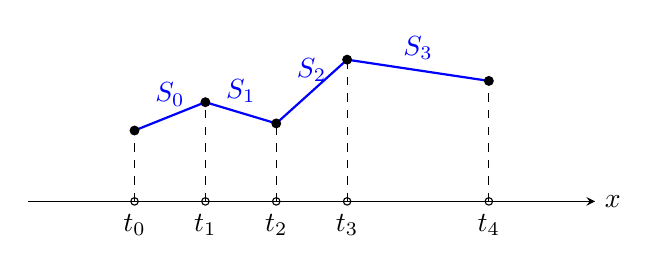
\begin{tikzpicture}[scale=0.9,>=stealth]
% Axis
\draw[->] (-1.5,0) -- (6.5,0) node[right] {$x$};

% Knot positions
\foreach \x/\label in {0/t_0,1/t_1,2/t_2,3/t_3,5/t_4} {
    \draw (\x,0) circle (1.5pt);
    \node[below] at (\x,-0.05) {$\label$};
}

% Points (ti, yi)
\coordinate (P0) at (0,1);
\coordinate (P1) at (1,1.4);
\coordinate (P2) at (2,1.1);
\coordinate (P3) at (3,2.0);
\coordinate (P4) at (5,1.7);

% Vertical dashed lines
\foreach \p in {P0,P1,P2,P3,P4} {
    \draw[dashed] (\p |- 0,0) -- (\p);
}

% Spline segments
\draw[thick,blue] (P0) -- (P1) node[midway,above] {$S_0$};
\draw[thick,blue] (P1) -- (P2) node[midway,above] {$S_1$};
\draw[thick,blue] (P2) -- (P3) node[midway,above] {$S_2$};
\draw[thick,blue] (P3) -- (P4) node[midway,above] {$S_3$};

% Data points
\foreach \p in {P0,P1,P2,P3,P4} {
    \fill (\p) circle (2pt);
}
\end{tikzpicture}
\end{center}

\begin{itemize}
    \item The issue with a first degree polynomial is the \textit{smoothness}
    \item Splines have applications in graphics 
\end{itemize}

\keyidea{We need to increase the degree of the polynomial for visual smoothness.}
\end{frame}

    

%%%%%%%%%%%%%%%%%%%%%%%%%%%%%%%%%%%%%%%%%%%%%%%%%%%%%%%%%%%%%%%%%%%%%%%%
\sectionframe{Second-Degree Spline}
%%%%%%%%%%%%%%%%%%%%%%%%%%%%%%%%%%%%%%%%%%%%%%%%%%%%%%%%%%%%%%%%%%%%%%%%

\begin{frame}{Second-Degree Spline}

\define{Second-Degree Spline}{
A function $S(x)$ is a \textbf{spline of degree 2} if all conditions are satisfied:
\begin{enumerate}
  \item The domain of $S(x)$ is an interval $[a,b]$
  \item $S(x)$ is continuous on $[a,b]$
  \item $S'(x)$ is continuous on $[a,b]$
  \item There is a partition $a=t_0<t_1<\dots<t_n=b$ such that $S(x)$ is
\emph{quadratic} on each subinterval $[t_i,t_{i+1}]$.
\end{enumerate}
}

Second degree splines have the form
\begin{equation*}
  S(x) = \begin{cases}
  S_0(x) &  x\in[t_0,t_1]\\
  S_1(x) &  x\in[t_1,t_2]\\
  \vdots & \vdots \\
  S_{n-1}(x) &  x\in[t_{n-1},t_n]\\
\end{cases},\quad   S_i(x) = a_i x^2 + b_i x + c_i
\end{equation*}

\end{frame}
%%%%%%%%%%%%%%%%%%%%%%%%%%%%%%%%%%%%%%%%%%%%%%%%%%%%%%%%%%%%%%%%%%%%%%%%
\begin{frame}{Is this a second-degree spline?}
\begin{center}
    
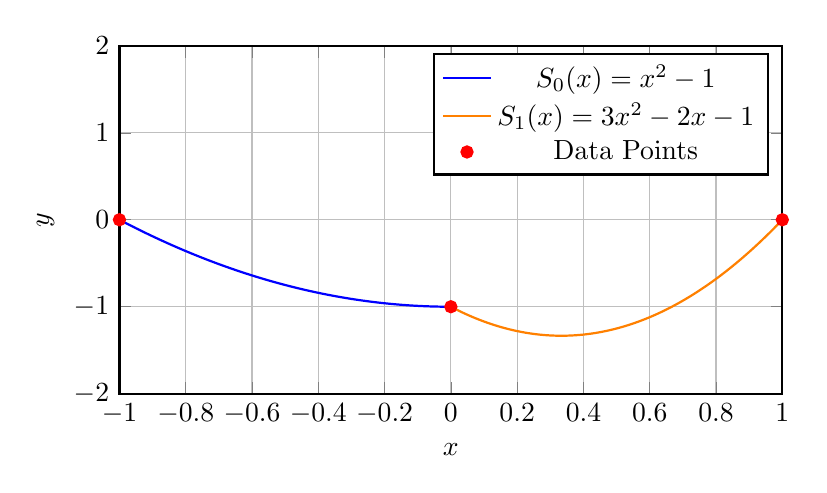
\begin{tikzpicture}
    \begin{axis}[
        width=10cm, height=6cm,
        xlabel={$x$}, ylabel={$y$},
        grid=major, 
        thick,
        xmin=-1, xmax=1,
        ymin=-2, ymax=2,
        samples=100,
    ]
    % Quadratic spline segment s0(x) for [-1, 0]
    \addplot[color=blue, thick, domain=-1:0] {x^2-1}; % Example function for s0(x)

    % Quadratic spline segment s1(x) for [0, 1]
    \addplot[color=orange, thick, domain=0:1] {3*x^2 -2*x -1}; % Example function for s1(x)

    % Data points
    \addplot[color=red, only marks, mark=*] 
        coordinates {(-1, 0) (0, -1) (1, 0)};
    
    % Optional legend
    \legend{$S_0(x)=x^2 - 1$, $S_1(x) = 3x^2 - 2x - 1$, Data Points};
    \end{axis}
\end{tikzpicture}\\
\begin{itemize}
    \item Each component is a quadratic $\checkmark$
    \item $S(x)$ is continuous $\checkmark$
\end{itemize}
\question{What's the problem here?}
\end{center}
\end{frame}

%%%%%%%%%%%%%%%%%%%%%%%%%%%%%%%%%%%%%%%%%%%%%%%%%%%%%%%%%%%%%%%%%%%%%%%%
\begin{frame}{Smoothness}
\begin{center}
    
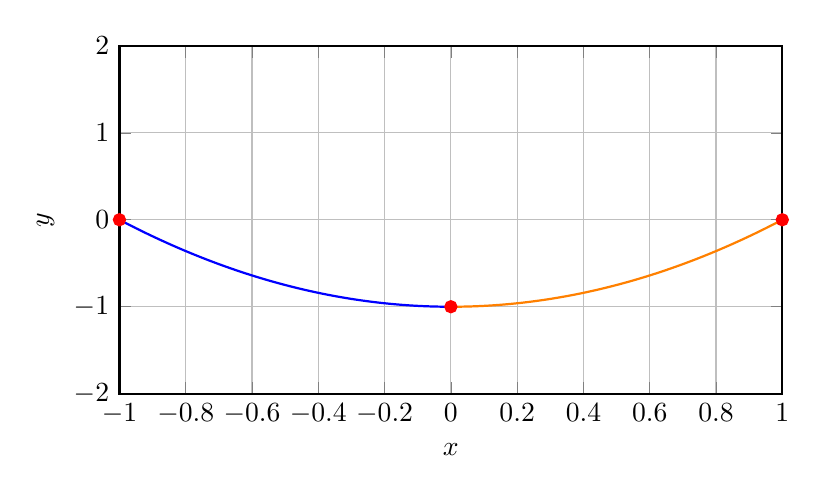
\begin{tikzpicture}
    \begin{axis}[
        width=10cm, height=6cm,
        xlabel={$x$}, ylabel={$y$},
        grid=major, 
        thick,
        xmin=-1, xmax=1,
        ymin=-2, ymax=2,
        samples=100,
    ]
    % Quadratic spline segment s0(x) for [-1, 0]
    \addplot[color=blue, thick, domain=-1:0] {x^2-1}; % Example function for s0(x)
    % Quadratic spline segment s1(x) for [0, 1]
    \addplot[color=orange, thick, domain=0:1] {x^2 -1}; % Example function for s1(x)
    % Data points
    \addplot[color=red, only marks, mark=*] 
        coordinates {(-1, 0) (0, -1) (1, 0)};
    \end{axis}
\end{tikzpicture}

\keyidea{
 Unlike degree 1 splines, degree 2 splines must be smooth
}
\end{center}
\end{frame}

%%%%%%%%%%%%%%%%%%%%%%%%%%%%%%%%%%%%%%%%%%%%%%%%%%%%%%%%%%%%%%%%%%%

\begin{frame}{Smoothness Condition}
\begin{center}
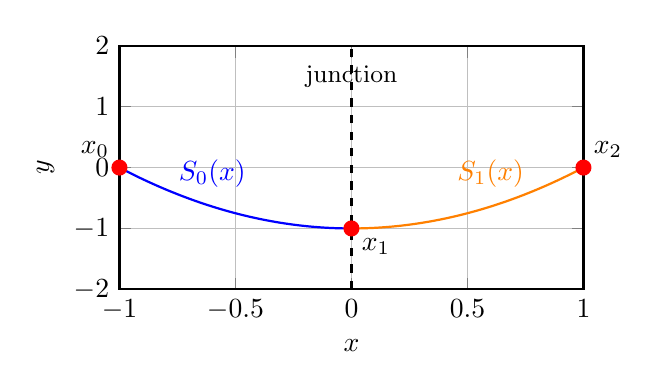
\begin{tikzpicture}
\begin{axis}[
    scale=0.7,
    width=10cm, height=6cm,
    xlabel={$x$}, ylabel={$y$},
    grid=major, 
    thick,
    xmin=-1, xmax=1,
    ymin=-2, ymax=2,
    samples=100,
    clip=false
]

% Left spline S0
\addplot[color=blue, thick, domain=-1:0] {x^2-1};
\node[blue,above] at (axis cs:-0.6,-0.5) {$S_0(x)$};

% Right spline S1
\addplot[color=orange, thick, domain=0:1] {x^2-1};
\node[orange,above] at (axis cs:0.6,-0.5) {$S_1(x)$};

% Data points
\addplot[color=red, only marks, mark=*, mark size=2.5pt] 
    coordinates {(-1, 0) (0, -1) (1, 0)};

% Label nodes
\node[above left] at (axis cs:-1,0) {$x_0$};
\node[below right] at (axis cs:0,-1) {$x_1$};
\node[above right] at (axis cs:1,0) {$x_2$};

% Highlight the junction
\draw[dashed] (axis cs:0,-2) -- (axis cs:0,2);
\node at (axis cs:0,1.5) {\small junction};

% Indicate matching slope
% \draw[->, thick] (axis cs:-0.15,-1.2) -- (axis cs:0,-1);
% \draw[->, thick] (axis cs:0.15,-1.2) -- (axis cs:0,-1);

% \node at (axis cs:0,-1.5) {\small matching slope};

\end{axis}
\end{tikzpicture}
\end{center}

\begin{itemize}
    \item The node $x_1$ separates the spline pieces $S_0(x)$ and $S_1(x)$
    \item To enforce smoothness, we require matching derivatives
    $$
        S_0'(x_1) = S_1'(x_1)
    $$
\end{itemize}

\end{frame}
%%%%%%%%%%%%%%%%%%%%%%%%%%%%%%%%%%%%%%%%%%%%%%%%%%%%%%%%%%%%%%%%%%%

\begin{frame}{Number of Unknowns}

\begin{center}
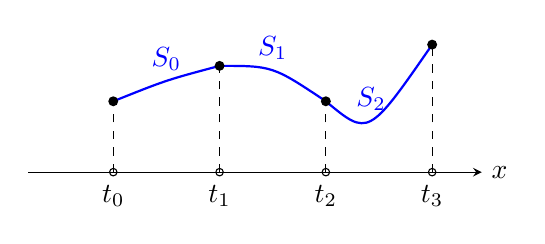
\begin{tikzpicture}[scale=0.9,>=stealth]
% Axis
\draw[->] (-1.2,0) -- (5.2,0) node[right] {$x$};
% Knot positions
\foreach \x/\label in {0/t_0,1.5/t_1,3/t_2,4.5/t_3} {
    \draw (\x,0) circle (1.5pt);
    \node[below] at (\x,-0.05) {$\label$};
}
% Data points
\coordinate (P0) at (0,1.0);
\coordinate (P1) at (1.5,1.5);
\coordinate (P2) at (3.0,1.0);
\coordinate (P3) at (4.5,1.8);
% Vertical dashed lines
\foreach \p in {P0,P1,P2,P3} {
    \draw[dashed] (\p |- 0,0) -- (\p);
}
% Quadratic spline segments (schematic curves)
\draw[thick,blue]
    (P0) .. controls (0.75,1.3) .. (P1)
    node[midway,above] {$S_0$};

\draw[thick,blue]
    (P1) .. controls (2.25,1.5) .. (P2)
    node[midway,above] {$S_1$};

\draw[thick,blue]
    (P2) .. controls (3.6,0.5) .. (P3)
    node[midway,above] {$S_2$};
% Data points
\foreach \p in {P0,P1,P2,P3} {
    \fill (\p) circle (2pt);
}
\end{tikzpicture}
\end{center}
\begin{itemize}
    \item Since each component has the form $S_i(x) = a_i x^2 + b_i x + c_i$, each have 3 unknown coefficients 
    \item If there are $n$ of them then there are 
    $$
    3\times3=\textbf{9 unknowns} 
    $$
    for a spline of degree 2
\end{itemize}

\end{frame}

%%%%%%%%%%%%%%%%%%%%%%%%%%%%%%%%%%%%%%%%%%%%%%%%%%%%%%%%%%%%%%%%%%%%%%%%

\begin{frame}{Number of Constraints}
\begin{center}
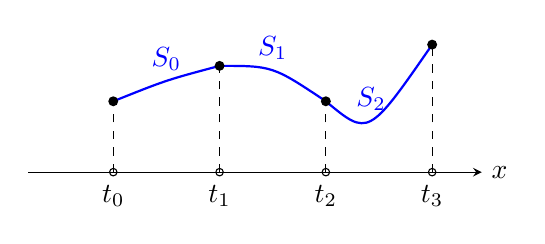
\begin{tikzpicture}[scale=0.9,>=stealth]
% Axis
\draw[->] (-1.2,0) -- (5.2,0) node[right] {$x$};
% Knot positions
\foreach \x/\label in {0/t_0,1.5/t_1,3/t_2,4.5/t_3} {
    \draw (\x,0) circle (1.5pt);
    \node[below] at (\x,-0.05) {$\label$};
}
% Data points
\coordinate (P0) at (0,1.0);
\coordinate (P1) at (1.5,1.5);
\coordinate (P2) at (3.0,1.0);
\coordinate (P3) at (4.5,1.8);
% Vertical dashed lines
\foreach \p in {P0,P1,P2,P3} {
    \draw[dashed] (\p |- 0,0) -- (\p);
}
% Quadratic spline segments (schematic curves)
\draw[thick,blue]
    (P0) .. controls (0.75,1.3) .. (P1)
    node[midway,above] {$S_0$};

\draw[thick,blue]
    (P1) .. controls (2.25,1.5) .. (P2)
    node[midway,above] {$S_1$};

\draw[thick,blue]
    (P2) .. controls (3.6,0.5) .. (P3)
    node[midway,above] {$S_2$};
% Data points
\foreach \p in {P0,P1,P2,P3} {
    \fill (\p) circle (2pt);
}
\end{tikzpicture}
\end{center}
\begin{itemize}
    \item For each component $S_i(x)$  must satisfy endpoints so there are 
    $$3 \times 2 = \textbf{6 constraints}$$
    \item We require smoothness at the \textbf{two interior nodes} where quadratics meet
    $$
    S'_0(t_1) = S_1'(t_1), \quad S_1'(t_2) = S_2'(t_2)
    $$
    \item Total constraints is 
        $$ 6 + 2 = \textbf{8 constraints}$$
\end{itemize}
\end{frame}

%%%%%%%%%%%%%%%%%%%%%%%%%%%%%%%%%%%%%%%%%%%%%%%%%%%%%%%%%%%%%%%%%%%%%

\begin{frame}{Constraints vs. Unknowns}
\begin{center}
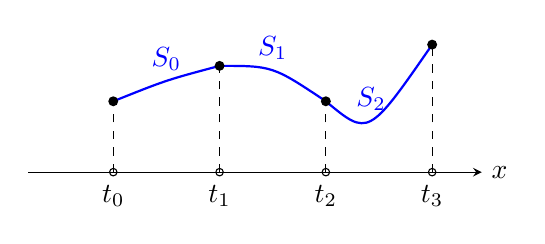
\begin{tikzpicture}[scale=0.9,>=stealth]
% Axis
\draw[->] (-1.2,0) -- (5.2,0) node[right] {$x$};
% Knot positions
\foreach \x/\label in {0/t_0,1.5/t_1,3/t_2,4.5/t_3} {
    \draw (\x,0) circle (1.5pt);
    \node[below] at (\x,-0.05) {$\label$};
}
% Data points
\coordinate (P0) at (0,1.0);
\coordinate (P1) at (1.5,1.5);
\coordinate (P2) at (3.0,1.0);
\coordinate (P3) at (4.5,1.8);
% Vertical dashed lines
\foreach \p in {P0,P1,P2,P3} {
    \draw[dashed] (\p |- 0,0) -- (\p);
}
% Quadratic spline segments (schematic curves)
\draw[thick,blue]
    (P0) .. controls (0.75,1.3) .. (P1)
    node[midway,above] {$S_0$};

\draw[thick,blue]
    (P1) .. controls (2.25,1.5) .. (P2)
    node[midway,above] {$S_1$};

\draw[thick,blue]
    (P2) .. controls (3.6,0.5) .. (P3)
    node[midway,above] {$S_2$};
% Data points
\foreach \p in {P0,P1,P2,P3} {
    \fill (\p) circle (2pt);
}
\end{tikzpicture}
\end{center}
\begin{itemize}
    \item Number of unknowns: $9$
    \item Number of constraints: $8$
    \item<2-> \textbf{We are one constraint short}
    \item<3> Just make one up!
    $$S_0''(t_0)=0$$
\end{itemize}
\end{frame}


%%%%%%%%%%%%%%%%%%%%%%%%%%%%%%%%%%%%%%%%%%%%%%%%%%%%%%%%%%%%%%%%%%%%%

\begin{frame}{General Second-Degree Splines}

\begin{block}{Counting Unknowns}
\begin{itemize}
    \item There are $n$ subintervals and each piece is \emph{quadratic}:
    \[
        S_i(x) = a_i x^2 + b_i x + c_i
    \]
    \item This gives \textbf{$3n$ unknown coefficients}
\end{itemize}
\end{block}

\begin{block}{Counting Constraints}
\begin{itemize}
    \item Components must interpolate two endpoints which gives \textbf{$2n$ equations}
    \item Smoothness at the interior points gives us \textbf{$n-1$ equations}
    \item Total is \textbf{$3n-1$ constraints}
\end{itemize}
\end{block}


\keyidea{
\begin{itemize}
    \item Second-degree splines are \textbf{NOT} unique
    \item We need \textbf{ONE} extra condition such as $S'_0(t_0)=0$ or $S''_0(t_0)=0$
\end{itemize}
}
\end{frame}
%%%%%%%%%%%%%%%%%%%%%%%%%%%%%%%%%%%%%%%%%%%%%%%%%%%%%%%%%%%%%%%%%%%%%%
\sectionframe{Summary}
%%%%%%%%%%%%%%%%%%%%%%%%%%%%%%%%%%%%%%%%%%%%%%%%%%%%%%%%%%%%%%%%%%%%%%

\begin{frame}{What is Runge's phenomenon?}

\begin{figure}
    \centering
    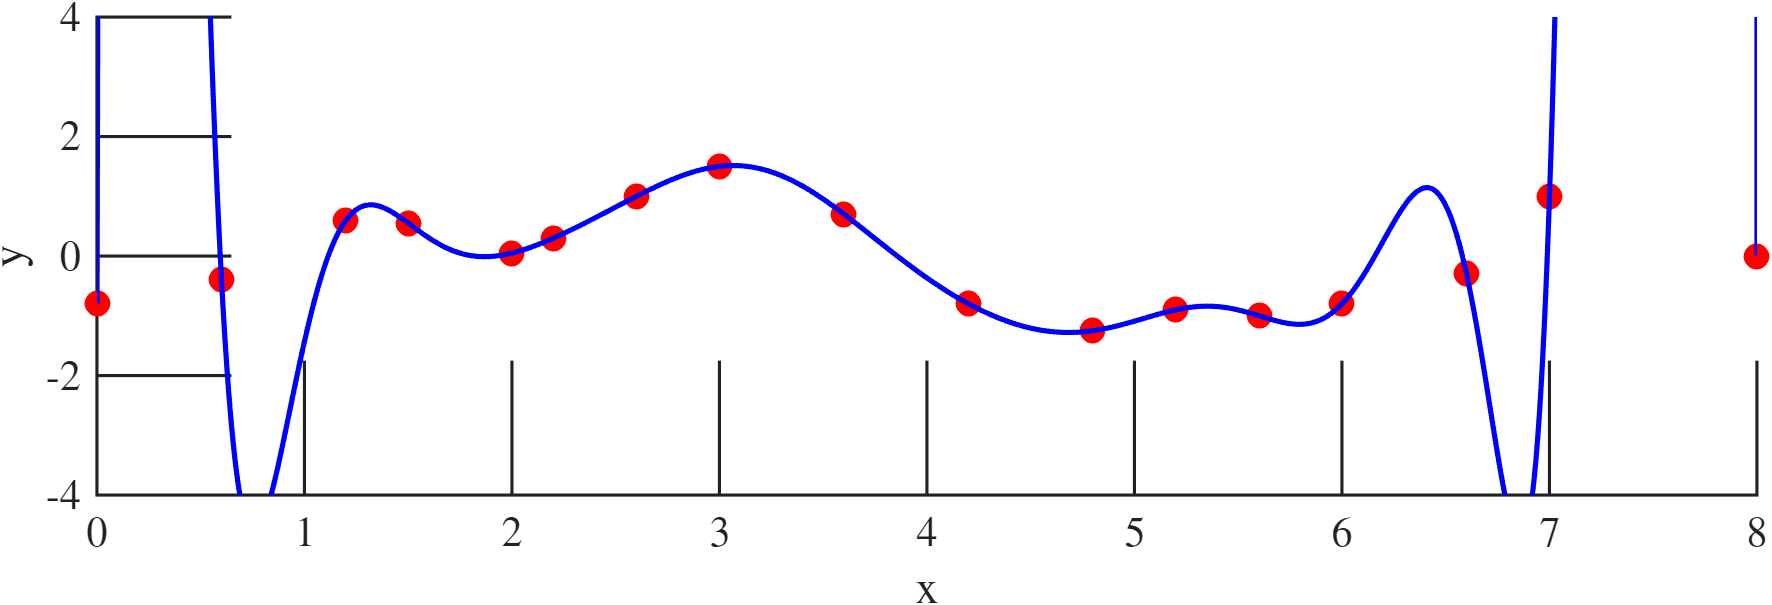
\includegraphics[width=0.8\linewidth]{figs/problem1b.png}
\end{figure}
    \begin{itemize}
        \item \textbf{Runge's phenomenon} is a notorious polynomial interpolation issue

        \item There are large fluctuations at the endpoints 
    \end{itemize}
\end{frame}

%%%%%%%%%%%%%%%%%%%%%%%%%%%%%%%%%%%%%%%%%%%%%%%%%%%%%%%%%%%%%%%%%%%%%%
\begin{frame}{What are Splines?}
    \begin{center}
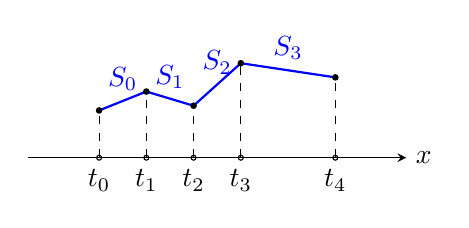
\begin{tikzpicture}[scale=0.6,>=stealth]
% Axis
\draw[->] (-1.5,0) -- (6.5,0) node[right] {$x$};

% Knot positions
\foreach \x/\label in {0/t_0,1/t_1,2/t_2,3/t_3,5/t_4} {
    \draw (\x,0) circle (1.5pt);
    \node[below] at (\x,-0.05) {$\label$};
}

% Points (ti, yi)
\coordinate (P0) at (0,1);
\coordinate (P1) at (1,1.4);
\coordinate (P2) at (2,1.1);
\coordinate (P3) at (3,2.0);
\coordinate (P4) at (5,1.7);

% Vertical dashed lines
\foreach \p in {P0,P1,P2,P3,P4} {
    \draw[dashed] (\p |- 0,0) -- (\p);
}

% Spline segments
\draw[thick,blue] (P0) -- (P1) node[midway,above] {$S_0$};
\draw[thick,blue] (P1) -- (P2) node[midway,above] {$S_1$};
\draw[thick,blue] (P2) -- (P3) node[midway,above] {$S_2$};
\draw[thick,blue] (P3) -- (P4) node[midway,above] {$S_3$};

% Data points
\foreach \p in {P0,P1,P2,P3,P4} {
    \fill (\p) circle (2pt);
}
\end{tikzpicture}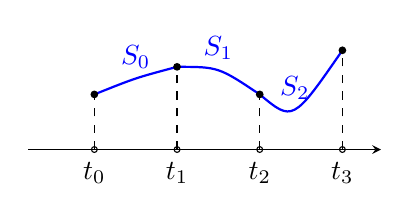
\begin{tikzpicture}[scale=0.7,>=stealth]
% Axis
\draw[->] (-1.2,0) -- (5.2,0);
% Knot positions
\foreach \x/\label in {0/t_0,1.5/t_1,3/t_2,4.5/t_3} {
    \draw (\x,0) circle (1.5pt);
    \node[below] at (\x,-0.05) {$\label$};
}
% Data points
\coordinate (P0) at (0,1.0);
\coordinate (P1) at (1.5,1.5);
\coordinate (P2) at (3.0,1.0);
\coordinate (P3) at (4.5,1.8);
% Vertical dashed lines
\foreach \p in {P0,P1,P2,P3} {
    \draw[dashed] (\p |- 0,0) -- (\p);
}
% Quadratic spline segments (schematic curves)
\draw[thick,blue]
    (P0) .. controls (0.75,1.3) .. (P1)
    node[midway,above] {$S_0$};

\draw[thick,blue]
    (P1) .. controls (2.25,1.5) .. (P2)
    node[midway,above] {$S_1$};

\draw[thick,blue]
    (P2) .. controls (3.6,0.5) .. (P3)
    node[midway,above] {$S_2$};
% Data points
\foreach \p in {P0,P1,P2,P3} {
    \fill (\p) circle (2pt);
}
\end{tikzpicture}
\end{center}
\begin{itemize}
    \item Splines are piecewise polynomial interpolations with smoothness conditions
    \item Each spline piece is a low-degree polynomial
\end{itemize}
\keyidea{Instead of one big high-degree polynomial, use multiple low-order polynomials.}
\end{frame}

%%%%%%%%%%%%%%%%%%%%%%%%%%
\begin{frame}{Counting Unknowns}
    \begin{itemize}
        \item Suppose there are $n+1$ data points. Then you have $n$ spline pieces.
        \vfill 
        \item Degree 1 Splines contain $2n$ unknowns because each piece is 
        $$
            S_i(x)=a_i x + b_i
        $$
        \vfill 
        \item Degree 2 Splines contain $3n$ unknowns because each piece is 
        $$
            S_i(x)=a_i x^2 + b_i x +c_i
        $$
    \end{itemize}
\end{frame}
%%%%%%%%%%%%%%%%%%%%%%%%%%
\begin{frame}{Uniqueness}
    \begin{itemize}
        \item Degree 1 splines require
        \begin{itemize}
            \item continuity: $2n$ conditions
        
        \end{itemize} 
        \vfill 
        \item Degree 2 Splines require 
        \begin{itemize}
            \item continuity: $2n$ conditions
            \item smoothness: $n-1$ conditions 
            \item total: $3n-1$ conditions
        \end{itemize}
    \end{itemize}
    \keyidea{
\begin{itemize}
    \item There is one unique degree 1 spline 
    \item Degree 2 splines are not unique because they are missing a condition
\end{itemize}
    }
\end{frame}
%%%%%%%%%%%%%%%%%%%
\begin{frame}{Moving Forward}
\begin{itemize}
    \item How to construct degree 2 splines by hand 
    \vfill 
    \item How to construct degree 2 splines efficiently
    \vfill
    \item Degree 3 splines
    \vfill 
    \item Cost of constructing degree splines
\end{itemize}
\end{frame}
\end{document}

